\documentclass[./\jobname.tex]{subfiles}
\begin{document}
%
\def\codeFolderName{deltasigma}
\def\codeFileName{ds_dac_sl}
\def\codeFolderNameB{}
%
\chapter{DAC}
%
\section{Einleitung}
%
Bei dieser Aufgabe soll ein \gls{dac} in Simulink erstellt und simuliert werden. Anschließend soll eine Verilog Codegenerierung gemacht werden. Die Verilog Codegenerierung benötigt \enquote{fixed-point} Datentypen, somit müssen die \enquote{double} Datentypen richtig deklariert werden. Dabei muss beachtet werden, dass bei Summen ein Überlauf stattfinden kann und somit das Ergebnis ein Bit länger sein muss wie die Eingänge.
%
\section{Implementierung}
%
Ein Delta-Sigma-Wandler wandelt einen digitalen Wert in einen Bitstrom um. Der Durchschnittswert des Bitstroms ist der digitale Eingabewert. Ein analoger Tiefpassfilter (Rekonstruktionsfilter) wird dann verwendet, um den Durchschnitt des Bitstroms zu erhalten. Dadurch wird der digitale Wert in ein analoges Signal (z. B. Spannung) umgewandelt.\par
%
In \autoref{fig: Simulink Implementierung} ist die Implementierung ersichtlich, bestehend aus:
%
\begin{description}
	\item[Signalgenerierung:] Vorgabe einer DC oder Sinus Spannung.
	\item[Diskretisierung mit Halteglied:] Hier wird das generierte Signal auf ein \enquote{digitales} Signal gewandelt.
	\item[\enquote{ds\_dac\_dbl}:] Hier wird der der Sigma Delta Wandler mit \enquote{double} Datentypen simuliert (siehe \autoref{fig: Simulink Implementierung 5}).
	\item[\enquote{ds\_dac\_sl}:] Hier wird der Sigma Delta Wandler mit \enquote{fixed-point} Datentypen simuliert und ist somit für die Verilog Codegenerierung geeignet (siehe \autoref{fig: Simulink Implementierung 6}).
	\item[\enquote{\gls{pwm}}:] Ist ein Vergleich, wie mit einer \gls{pwm} ein \enquote{analoges} Signal generiert werden kann.
	\item[DS\_DAC\_Trans\_XXX:] Hier wird ein Tiefpassfilter auf das generierte Pulssignal angewendet (siehe \autoref{fig: Simulink Implementierung 2}).
\end{description}
%
Die Samplezeit wurde auf \(\frac{1}{50\cdot 10^{6}}~s\) gestellt und ein Fixed-step Solver ausgewählt. \(\tau\) wurde \(0.01 \cdot 10^{-3}\) gewählt. Die Frequenz ist mit \(100~Hz\) definiert.
%
% T=1/50e6;
% tau = 0.01e-3;
%
\begin{figure}[H]
	\centering
	\noindent\adjustbox{max width=\textwidth}{%falls größer als \textwidth, wird das Bild verkleinert
		%trim option's parameter order: left bottom right top
		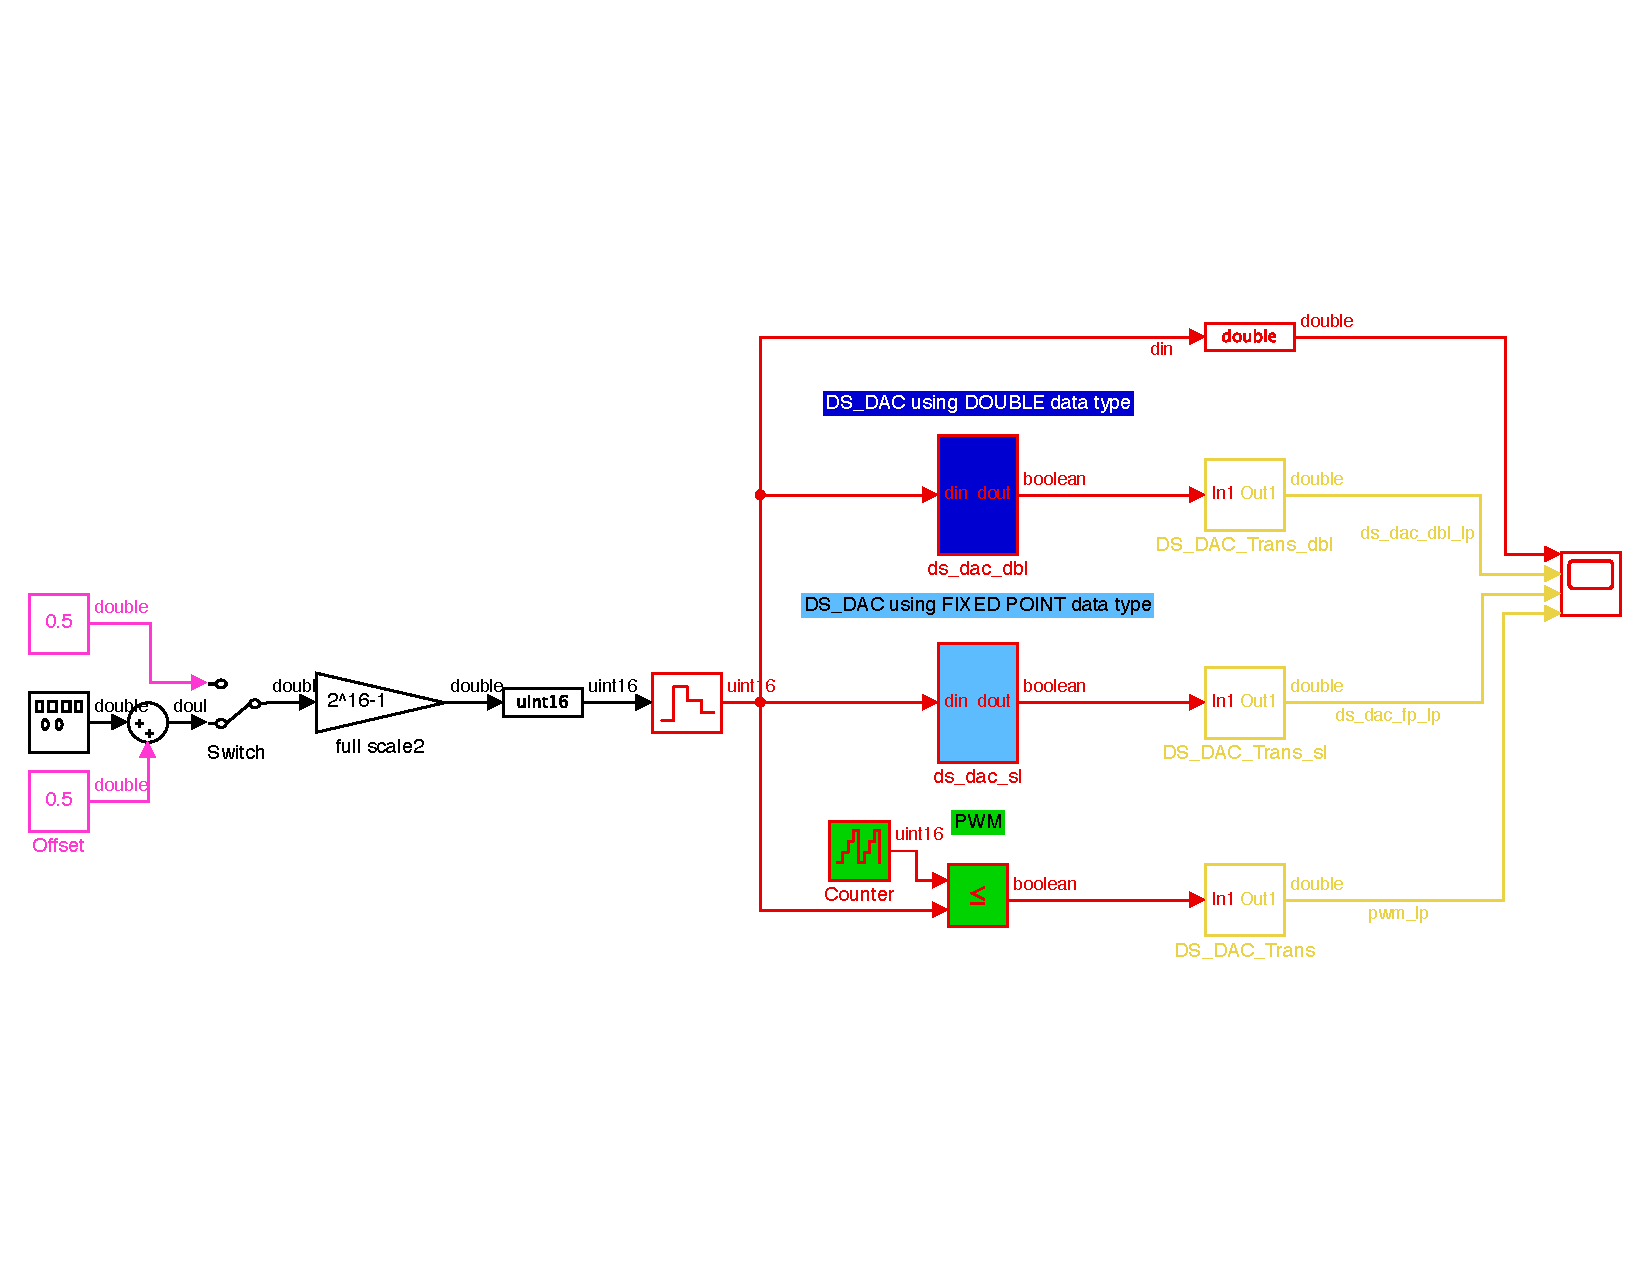
\includegraphics[width=1\textwidth,page=1]{./../code/\codeFolderName\codeFolderNameB/doc/simulink.pdf}
	}
	\unterschrift{Simulink Implementierung}{eigene Ausarbeitung}{}
	\label{fig: Simulink Implementierung}
\end{figure}
%
\begin{figure}[H]
	\centering
	\noindent\adjustbox{max width=\textwidth}{%falls größer als \textwidth, wird das Bild verkleinert
		%trim option's parameter order: left bottom right top
		\includegraphics[width=0.75\textwidth,page=2]{./../code/\codeFolderName\codeFolderNameB/doc/simulink.pdf}
	}
	\unterschrift{Simulink Implementierung: Tiefpassfilter}{eigene Ausarbeitung}{}
	\label{fig: Simulink Implementierung 2}
\end{figure}
%
%\begin{figure}[H]
%	\centering
%	\noindent\adjustbox{max width=\textwidth}{%falls größer als \textwidth, wird das Bild verkleinert
%		%trim option's parameter order: left bottom right top
%		\includegraphics[width=1\textwidth,page=3]{./../code/\codeFolderName\codeFolderNameB/doc/simulink.pdf}
%	}
%	\unterschrift{Simulink Implementierung}{eigene Ausarbeitung}{}
%	\label{fig: Simulink Implementierung 3}
%\end{figure}
%%
%\begin{figure}[H]
%	\centering
%	\noindent\adjustbox{max width=\textwidth}{%falls größer als \textwidth, wird das Bild verkleinert
%		%trim option's parameter order: left bottom right top
%		\includegraphics[width=1\textwidth,page=4]{./../code/\codeFolderName\codeFolderNameB/doc/simulink.pdf}
%	}
%	\unterschrift{Simulink Implementierung}{eigene Ausarbeitung}{}
%	\label{fig: Simulink Implementierung 4}
%\end{figure}
%
\begin{figure}[H]
	\centering
	\noindent\adjustbox{max width=\textwidth}{%falls größer als \textwidth, wird das Bild verkleinert
		%trim option's parameter order: left bottom right top
		\includegraphics[width=1\textwidth,page=5]{./../code/\codeFolderName\codeFolderNameB/doc/simulink.pdf}
	}
	\unterschrift{Simulink Implementierung: \glsentryshort{dac} mit \enquote{fixed-point} Datentypen}{eigene Ausarbeitung}{}
	\label{fig: Simulink Implementierung 5}
\end{figure}
%
\begin{figure}[H]
	\centering
	\noindent\adjustbox{max width=\textwidth}{%falls größer als \textwidth, wird das Bild verkleinert
		%trim option's parameter order: left bottom right top
		\includegraphics[width=1\textwidth,page=6]{./../code/\codeFolderName\codeFolderNameB/doc/simulink.pdf}
	}
	\unterschrift{Simulink Implementierung: \glsentryshort{dac} mit \enquote{double} Datentypen}{eigene Ausarbeitung}{}
	\label{fig: Simulink Implementierung 6}
\end{figure}
%
Bei der Verilog Codegenerierung ist ersichtlich, dass die Deklaration von Variablen noch genauer angeben ist. Es muss die Dateiendung von \enquote{*.s} auf \enquote{*.sv} geändert werden.
%
\lstinputlisting[language=Verilog,label={lst:counter_updn}, caption=Resultat der Codegenerierung]{./../code/\codeFolderName\codeFolderNameB/src/\codeFileName.sv}
%
\section{Test Bench}
%
In \autoref{lst:tb_counter_updn} ist die Testbench ersichtlich. Das Herzstück der Testbench ist die Sinusgenerierung (Codezeile \ref{code: sinusgenerierung}). Diese Anweisung verpackt in einer \enquote{while} Schleife ergibt einen Sinus. Die Frequenz, Amplitude und Startpunkt der Sinusgenerierung wurde zur besseren Vergleichbarkeit an die Simulation in Simulink angepasst.
%
\lstinputlisting[language=Verilog,label={lst:tb_counter_updn}, caption=Testbench für den \glsentryshort{dac}]{./../code/\codeFolderName\codeFolderNameB/sim/tb_\codeFileName.sv}
%
\section{Simulationsscript}
%
In \autoref{lst:sim_tb_counter_updn} ist das Simulationsscript dargestellt. Es beinhaltet dieselben Befehle wie in der letzten Lehrveranstaltung, natürlich angepasst an den \gls{dac}.
%
\lstinputlisting[language=tcl,label={lst:sim_tb_counter_updn}, caption=Simulationsscript]{./../code/\codeFolderName\codeFolderNameB/sim/sim_tb_\codeFileName.tcl}
%
\section{Waveform Window und Simulink Simulation}
%
In \autoref{fig: wavewindow_dac} ist das Waveform Window dargestellt. Es zeigt den generierten Sinus. In \autoref{fig: simulink} ist der Vergleich zur Simulation ersichtlich. Es ist ersichtlich, dass bei den \enquote{Peaks} (ca. bei \(2.5~ms\)) der Ausgang \enquote{High} und bei den \enquote{Lows} (ca. bei \(7.5~ms\)) der Ausgang \enquote{Low} ist.
%
\begin{figure}[H]
	\centering
	\noindent\adjustbox{max width=\textwidth}{%falls größer als \textwidth, wird das Bild verkleinert
		%trim option's parameter order: left bottom right top
	\includegraphics[width=1\textwidth]{./../code/\codeFolderName\codeFolderNameB/doc/wavewindow_\codeFileName.PNG}
	}
	\unterschrift{Waveform Window}{eigene Ausarbeitung}{}
	\label{fig: wavewindow_dac}
\end{figure}
%
\begin{figure}[H]
	\centering
	\noindent\adjustbox{max width=\textwidth}{%falls größer als \textwidth, wird das Bild verkleinert
		%trim option's parameter order: left bottom right top
		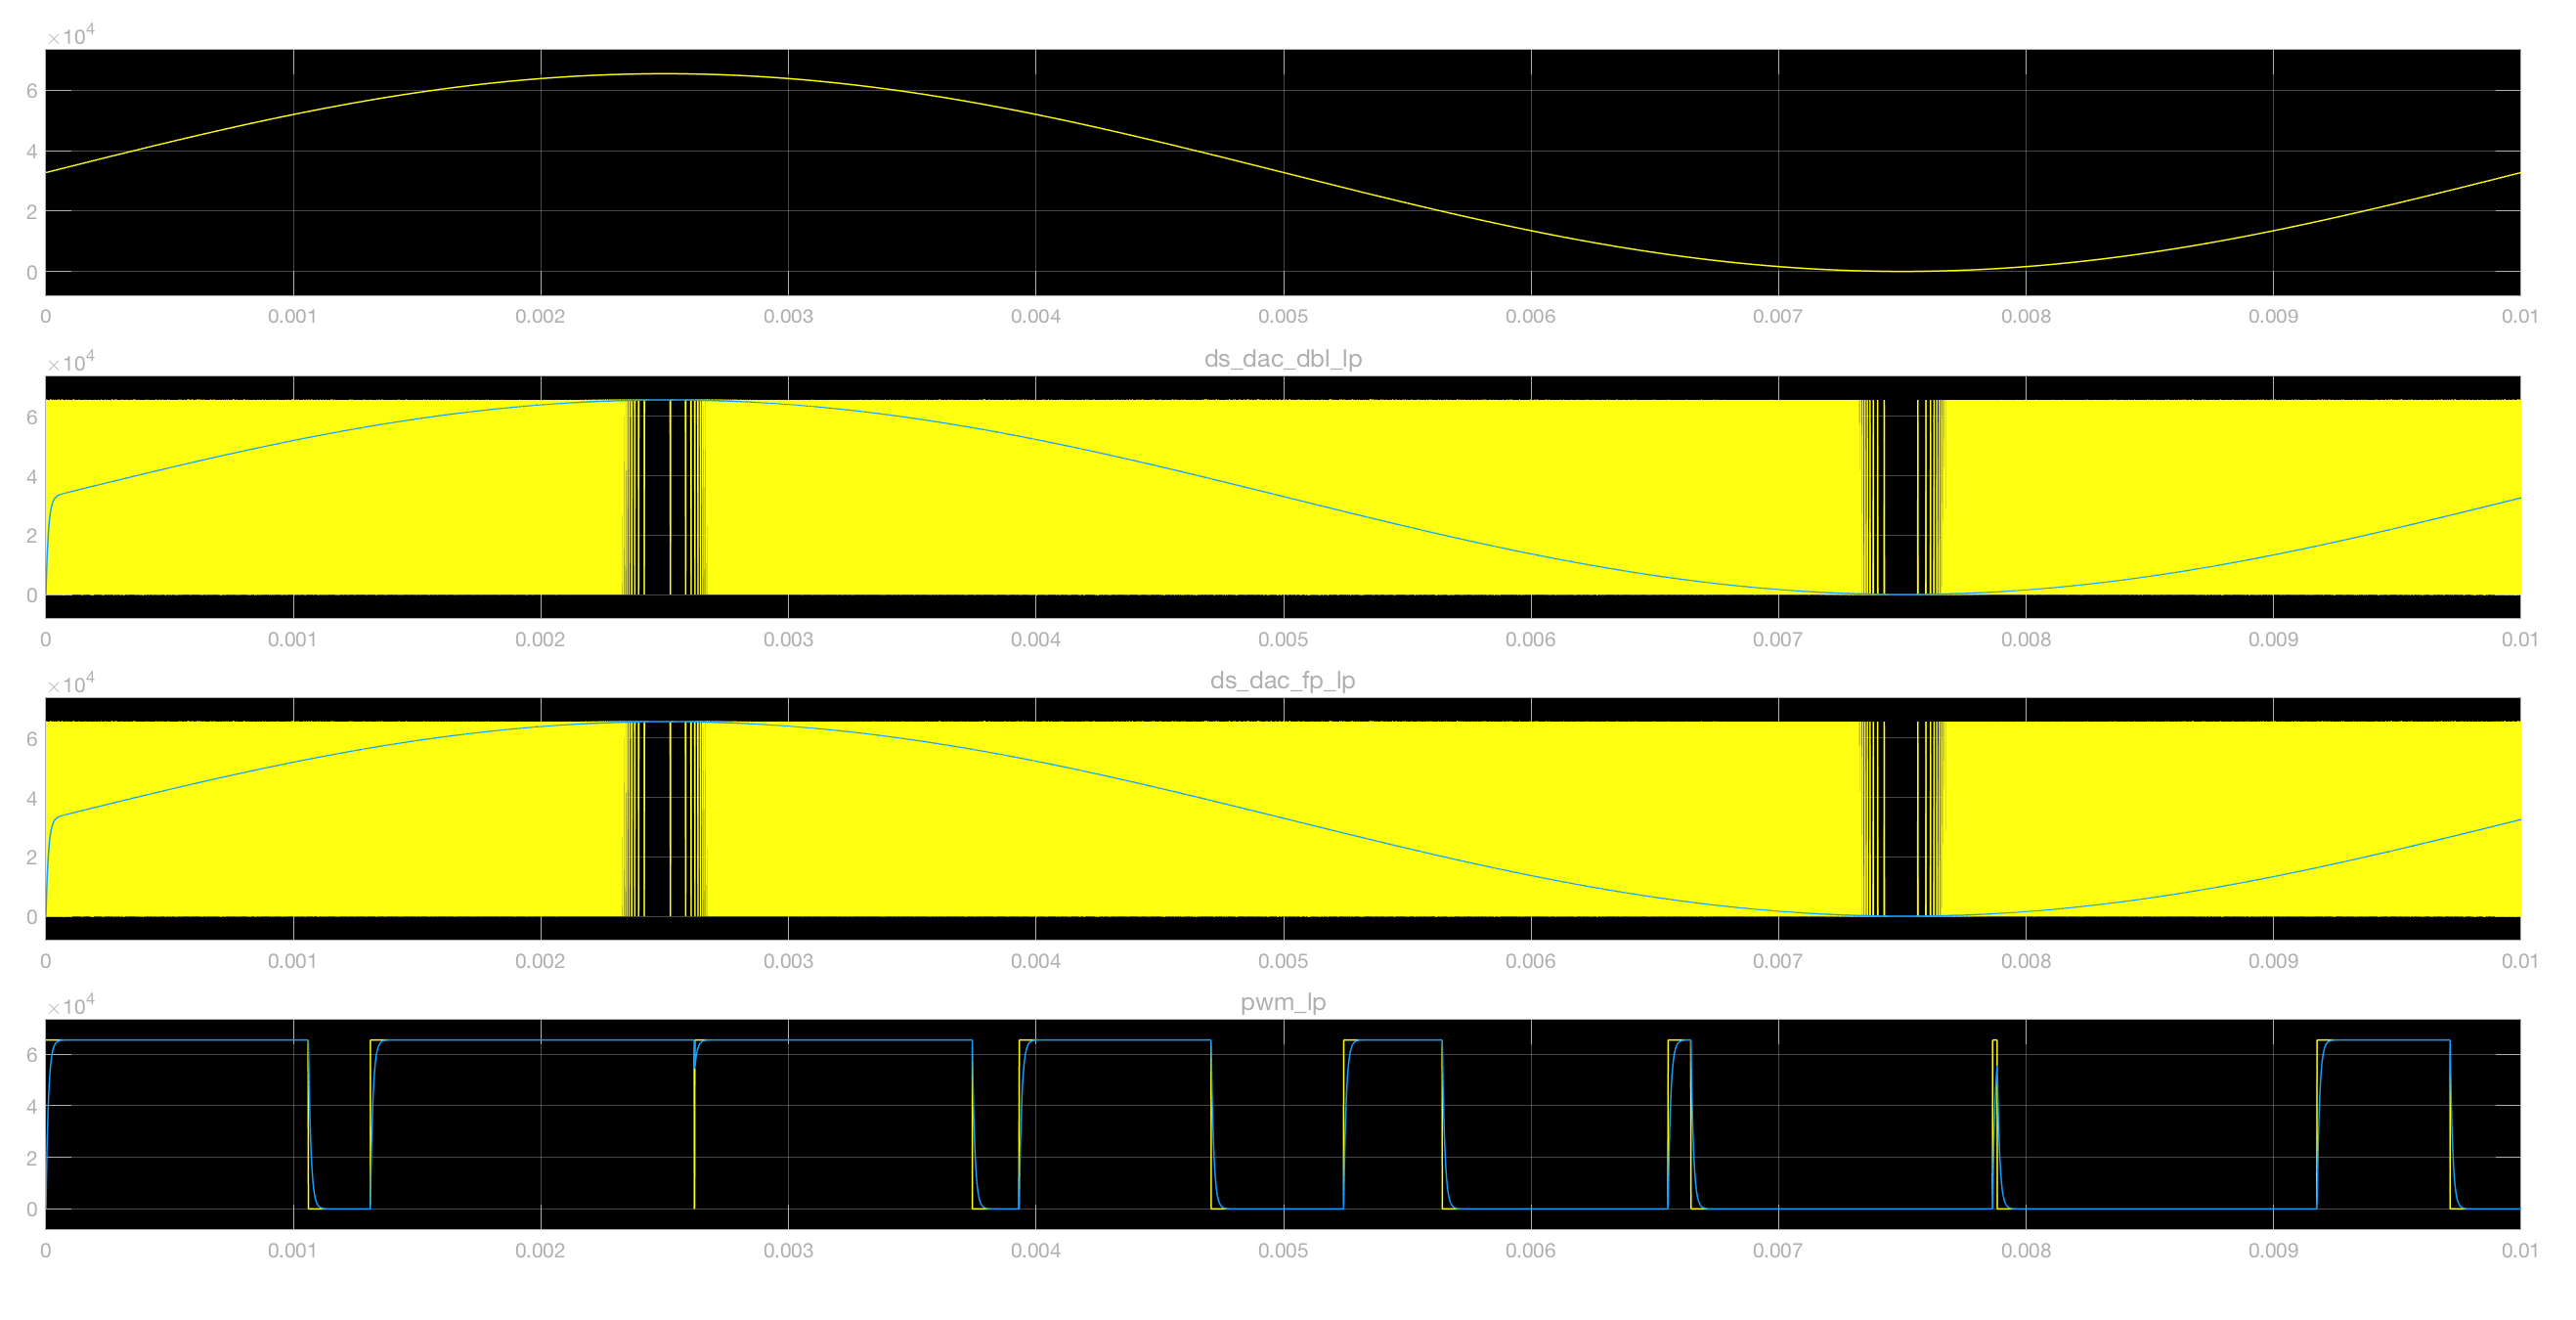
\includegraphics[width=1\textwidth]{./../code/\codeFolderName\codeFolderNameB/doc/simulink.eps}
	}
	\unterschrift{Simulink Simulationsergebnisse}{eigene Ausarbeitung}{}
	\label{fig: simulink}
\end{figure}
%
%In \autoref{ausgabeTwo} ist der Output des Testcripts zu sehen. Alle Testfälle wurden bestanden.
%%
%\lstinputlisting[language=tcl,
%label={ausgabeTwo}, caption=Commandline Output A]{./../code/counter_updn/doc/console_output.txt}
%
%\section{Vor- und Nachteile der Implementierung}
%%
%Folgend sind die Vor- und Nachteile der Implementierung gelistet:
%%
%\begin{description}
%	\item[Vorteile] \hfil
%	\begin{itemize}
%		\item Variable Bitlänge \pfeil Entprelldauer kann angepasst werden.
%	\end{itemize}
%	\item[Nachteile] \hfil
%	\begin{itemize}
%		\item Die Clock Frequenz darf nur so hoch gewählt werden, wie es das \enquote{Back Propagation Delay} erlaubt. Somit ist die maximale Zählfrequenz begrenzt.
%		\item Bei Anwahl des Down-Bits sollte beim Reseten der Counter Wert nicht auf \enquote{0} initalisiert werden, sondern mit dem maximalen Wert
%		\begin{align}
%		2~<<~ (`counterSize-1) - 1
%		\end{align}
%		\item Ebenfalls wäre es gut, den Startwert des Counters selbst wählen zu können.
%	\end{itemize}
%\end{description}
%
\end{document}
